\documentclass{beamer}

\usepackage[french]{babel}
\usepackage[T1]{fontenc}
\usepackage[utf8]{inputenc}
\usepackage{rotating}
\usepackage{array}

\usetheme{Warsaw}

\title[Provisionnement dynamique de serveurs de MMOG]{Provisionnement dynamique de serveurs de jeux massivement multijoueurs, approche par simulation}
\author{\underline{Guillaume Turchini}, Olivier Marin, Sébastien Monnet}
\institute{Présentation stage}
\date{Sept. 2015}

\setbeamertemplate{navigation symbols}{
}

\begin{document}

\begin{frame}
  \titlepage
\end{frame}

\setbeamertemplate{navigation symbols}{
  \usebeamerfont{footline}%
  \usebeamercolor[fg]{footline}%
  \hspace{1em}%
  \insertframenumber
}

\begin{frame}
  \frametitle{Contexte et Motivations}
  \begin{itemize}
    \item{Contraintes de performance strictes}
    \item{Grande échelle (millions de joueurs concurrents)}
    \item{Grande variation géographique à l'intérieur du monde de jeu (accès à des données différentes)}
    \item{Grande variation horaire du nombre de joueur}
  \end{itemize}
  \vspace{0.5cm}

  \centering
  \begin{tabular}{cc}
    \begin{sideways}\scriptsize{Nombre de joueurs}\end{sideways} &
    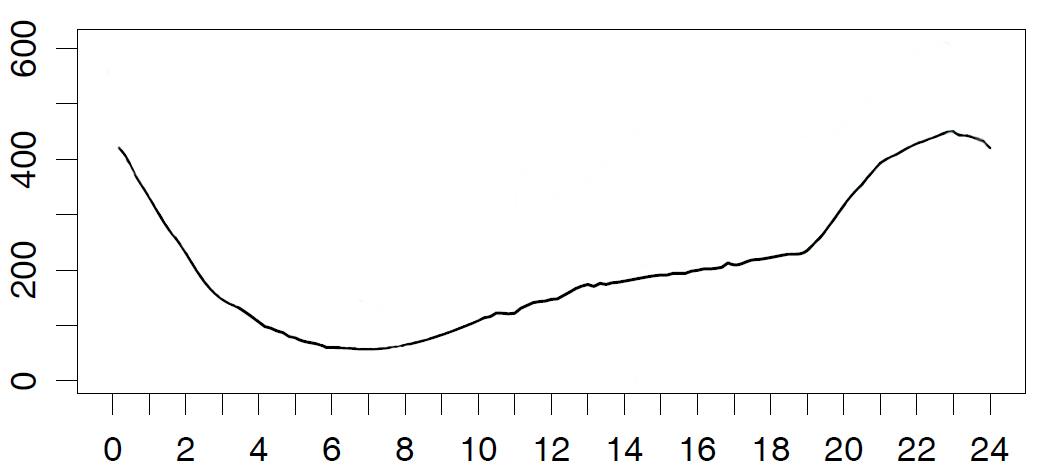
\includegraphics[width=5cm]{player_day_evol.png}\\
    & \scriptsize{Heure de la journée}
  \end{tabular}
  
  \scriptsize\textbf{Nombre moyen de joueurs connectés dans un royaume de World of Warcraft}\\
\end{frame}

\begin{frame}
  \frametitle{Problèmes de passage à l'échelle}
  \begin{itemize}
    \item{Un serveur = un nombre limité de joueurs
      \\[1mm]\hspace{1cm}$\Rightarrow$ Nécessité de partitionnement\vspace{5mm}}
    \item{Surdimentionnement de l'infrastructure
      \\[1mm]\hspace{1cm}$\Rightarrow$ Majoritairement vide}
  \end{itemize}
\end{frame}

\begin{frame}
  \frametitle{Méthodes de partitionnement}
  \begin{itemize}
    \item{Séparation en services}
    \item{Sharding\hspace{1cm}\raisebox{-0.5\height}{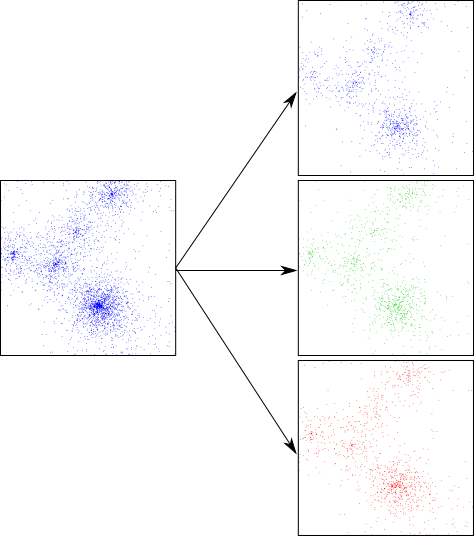
\includegraphics[width=3.4cm]{sharding.png}}}
    \item{Zoning\hspace{1cm}\raisebox{-0.5\height}{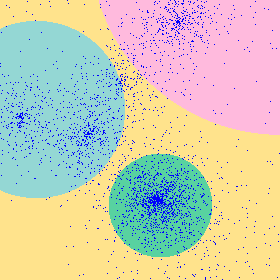
\includegraphics[width=1.8cm]{nuage_zonage.png}}}
    \item{Instancing}
    \item{Autres}
  \end{itemize}
\end{frame}

\begin{frame}
  \frametitle{Limites du partitionnement}
  \begin{itemize}
    \item{Sharding et Instancing
      \\[1mm]\hspace{1cm}$\Rightarrow$ Séparation des joueurs\vspace{5mm}}
    \item{Cloning et Time Slow
      \\[1mm]\hspace{1cm}$\Rightarrow$ Pas forcément applicable\vspace{5mm}}
    \item{Zoning avec frontières transparentes
      \\[1mm]\hspace{1cm}$\Rightarrow$ Seule approche générique possible}
  \end{itemize}
\end{frame}

\begin{frame}
  \frametitle{Architectures sur laquelle se base le partitionnement}
  \begin{itemize}
    \item{Client-Serveur\hspace{1cm}\raisebox{-0.5\height}{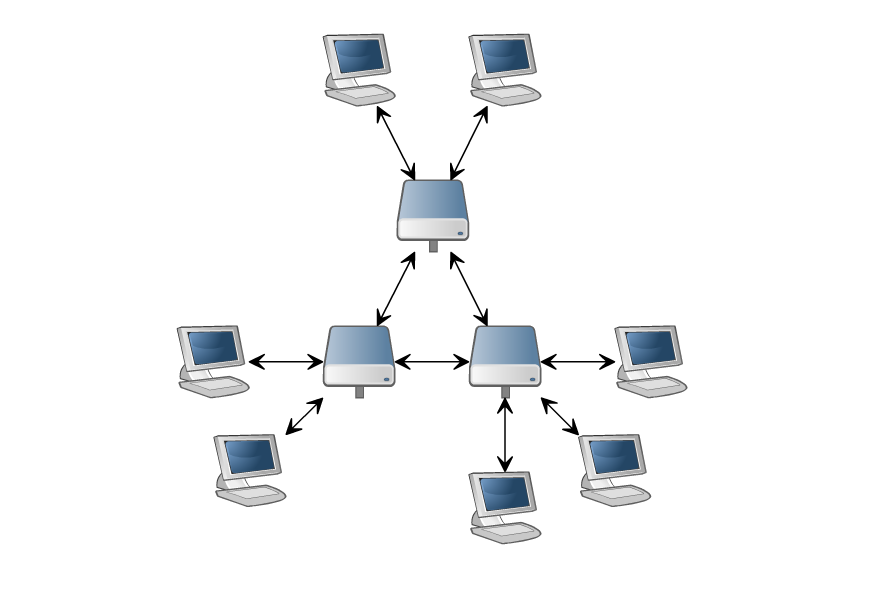
\includegraphics[width=4cm]{mcs.png}}}
    \item{Pair-à-Pair\hspace{1.5cm}\raisebox{-0.5\height}{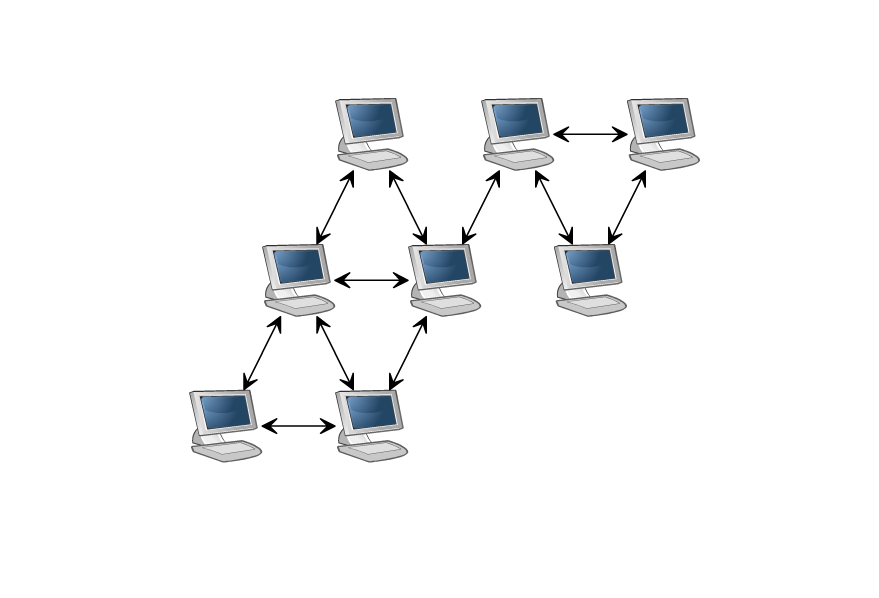
\includegraphics[width=4cm]{p2p.png}}}
  \end{itemize}
\end{frame}

\begin{frame}
  \frametitle{Architectures sur laquelle se base le partitionnement}
  \begin{itemize}
    \item{Hybride\vspace{5mm}}
    \item{GaaS\hspace{1cm}\raisebox{-0.5\height}{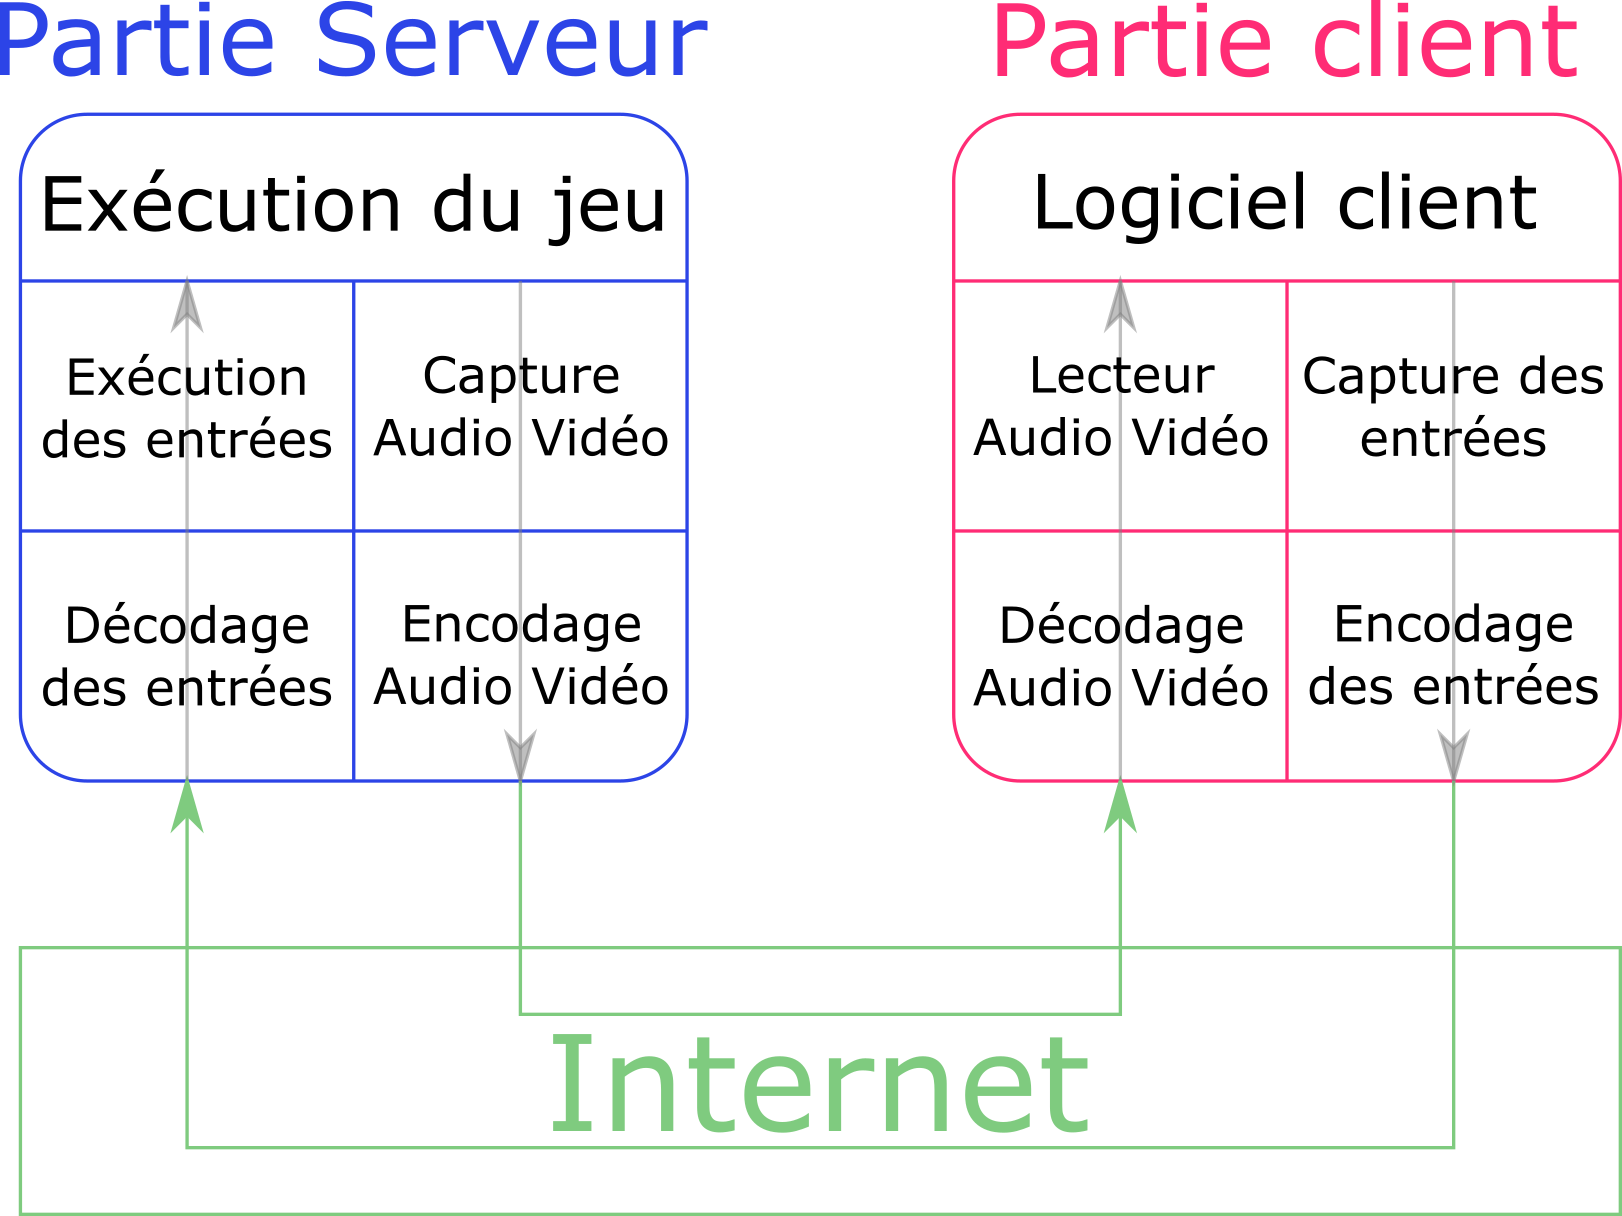
\includegraphics[width=5cm]{gaas.png}}}
  \end{itemize}
\end{frame}

\begin{frame}
  \frametitle{Métriques}
  \begin{itemize}
    \item{Latence}
    \item{Non respect de Tickrate}
    \item{Charge CPU}
    \item{Charge Réseau}
    \item{Charge Mémoire}
    \item{Prix de l'architecture (nombre de machines, temps d'utilisation et utilisation réseau)}
  \end{itemize}
\end{frame}

\begin{frame}
  \frametitle{Comparaison}
  \begin{center}
    \scriptsize
    \begin{tabular}{|>{\centering\arraybackslash}m{0.18\textwidth}|*{3}{>{\centering\arraybackslash}m{0.18\textwidth}|}}
      \hline
      
      ~&
      Client-Serveur&
      Client-Serveur\linebreak(multi-serveur)&
      Pair-à-Pair\\
      
      \hline
      
      Charge CPU&
      \'Elevée&
      Réduite&
      Chez le client\\
      
      \hline
      
      Charge Réseau&
      Normale&
      Entre serveurs\linebreak{}+\linebreak{}externe&
      Chez le client\\
      
      \hline
      
      Complexité de développement&
      Facile&
      Moyenne&
      Complexe\\
      
      \hline
      
      Coûts&
      Normaux&
      \'Elevés&
      Nuls\\
      
      \hline

      Latence&
      Normale&
      Normale&
      \'Elevée\\
      
      \hline
    \end{tabular}
  \end{center}
\end{frame}

\begin{frame}
  \normalsize
  \frametitle{Proposition}
  \begin{itemize}
    \item{Utiliser des VM dans le cloud}
    \begin{itemize}
      \item{\'Elasticité (Zonage dynamique)}
      \item{Nombre de machine et bande passante $\rightarrow\infty$}
      \item{Grande disponibilité}
    \end{itemize}
  \end{itemize}
\end{frame}

\begin{frame}
  \frametitle{Comparaison}
  \begin{center}
    \scriptsize
    \begin{tabular}{|>{\centering\arraybackslash}m{0.17\textwidth}|*{4}{>{\centering\arraybackslash}m{0.16\textwidth}|}}
      \hline
      
      ~&
      Client-Serveur&
      Client-Serveur\linebreak(multi-serveur)&
      Pair-à-Pair&
      Cloud\\
      
      \hline
      
      Charge CPU&
      \'Elevée&
      Réduite&
      Chez le client&
      Idem multi-serveur\\
      
      \hline
      
      Charge Réseau&
      Normale&
      Entre serveurs\linebreak{}+\linebreak{}externe&
      Chez le client&
      Idem multi-serveur\\
      
      \hline
      
      Complexité de développement&
      Facile&
      Moyenne&
      Complexe&
      Complexe\\
      
      \hline
      
      Coûts&
      Normaux&
      \'Elevés&
      Nuls&
      Moins élevés (?)\\
      
      \hline

      Latence&
      Normale&
      Normale&
      \'Elevée&
      Idem multi-serveur\\
      
      \hline
    \end{tabular}
  \end{center}
\end{frame}

\begin{frame}
  \normalsize
  \frametitle{Simulation}
  \begin{itemize}
    \item{Expérimentation dans le cloud}
    \begin{itemize}
      \item{Grande échelle}
      \item{Prix élevé}
      \item{Développement et Débuggage compliqué\vspace{5mm}}
    \end{itemize}
    \item{Approche par simulation}
    \begin{itemize}
      \item{Reproductibilité}
      \item{Gain de temps}
      \item{Débuggage plus simple (vue complète du système)\\[5mm]
        \hspace{5mm}$\Rightarrow$ Besoin d'un simulateur (contribution 1)}
    \end{itemize}
  \end{itemize}
\end{frame}

\begin{frame}
  \frametitle{Traces}
  \begin{itemize}
    \item{Traces existantes}
      \begin{itemize}
        \item{Imprécises}
        \item{Mauvaise échelle}
        \item{Nombre limité\\[0.5cm]\hspace{0.5cm}$\Rightarrow$ Générateur de traces (contribution 2)}
      \end{itemize}
  \end{itemize}
\end{frame}

\begin{frame}
  \frametitle{Modèle de mobilité}
  \begin{itemize}
    \item{Lévy's flight}
    \item{Hotspots (Blue Banana)\vspace{2mm}}
    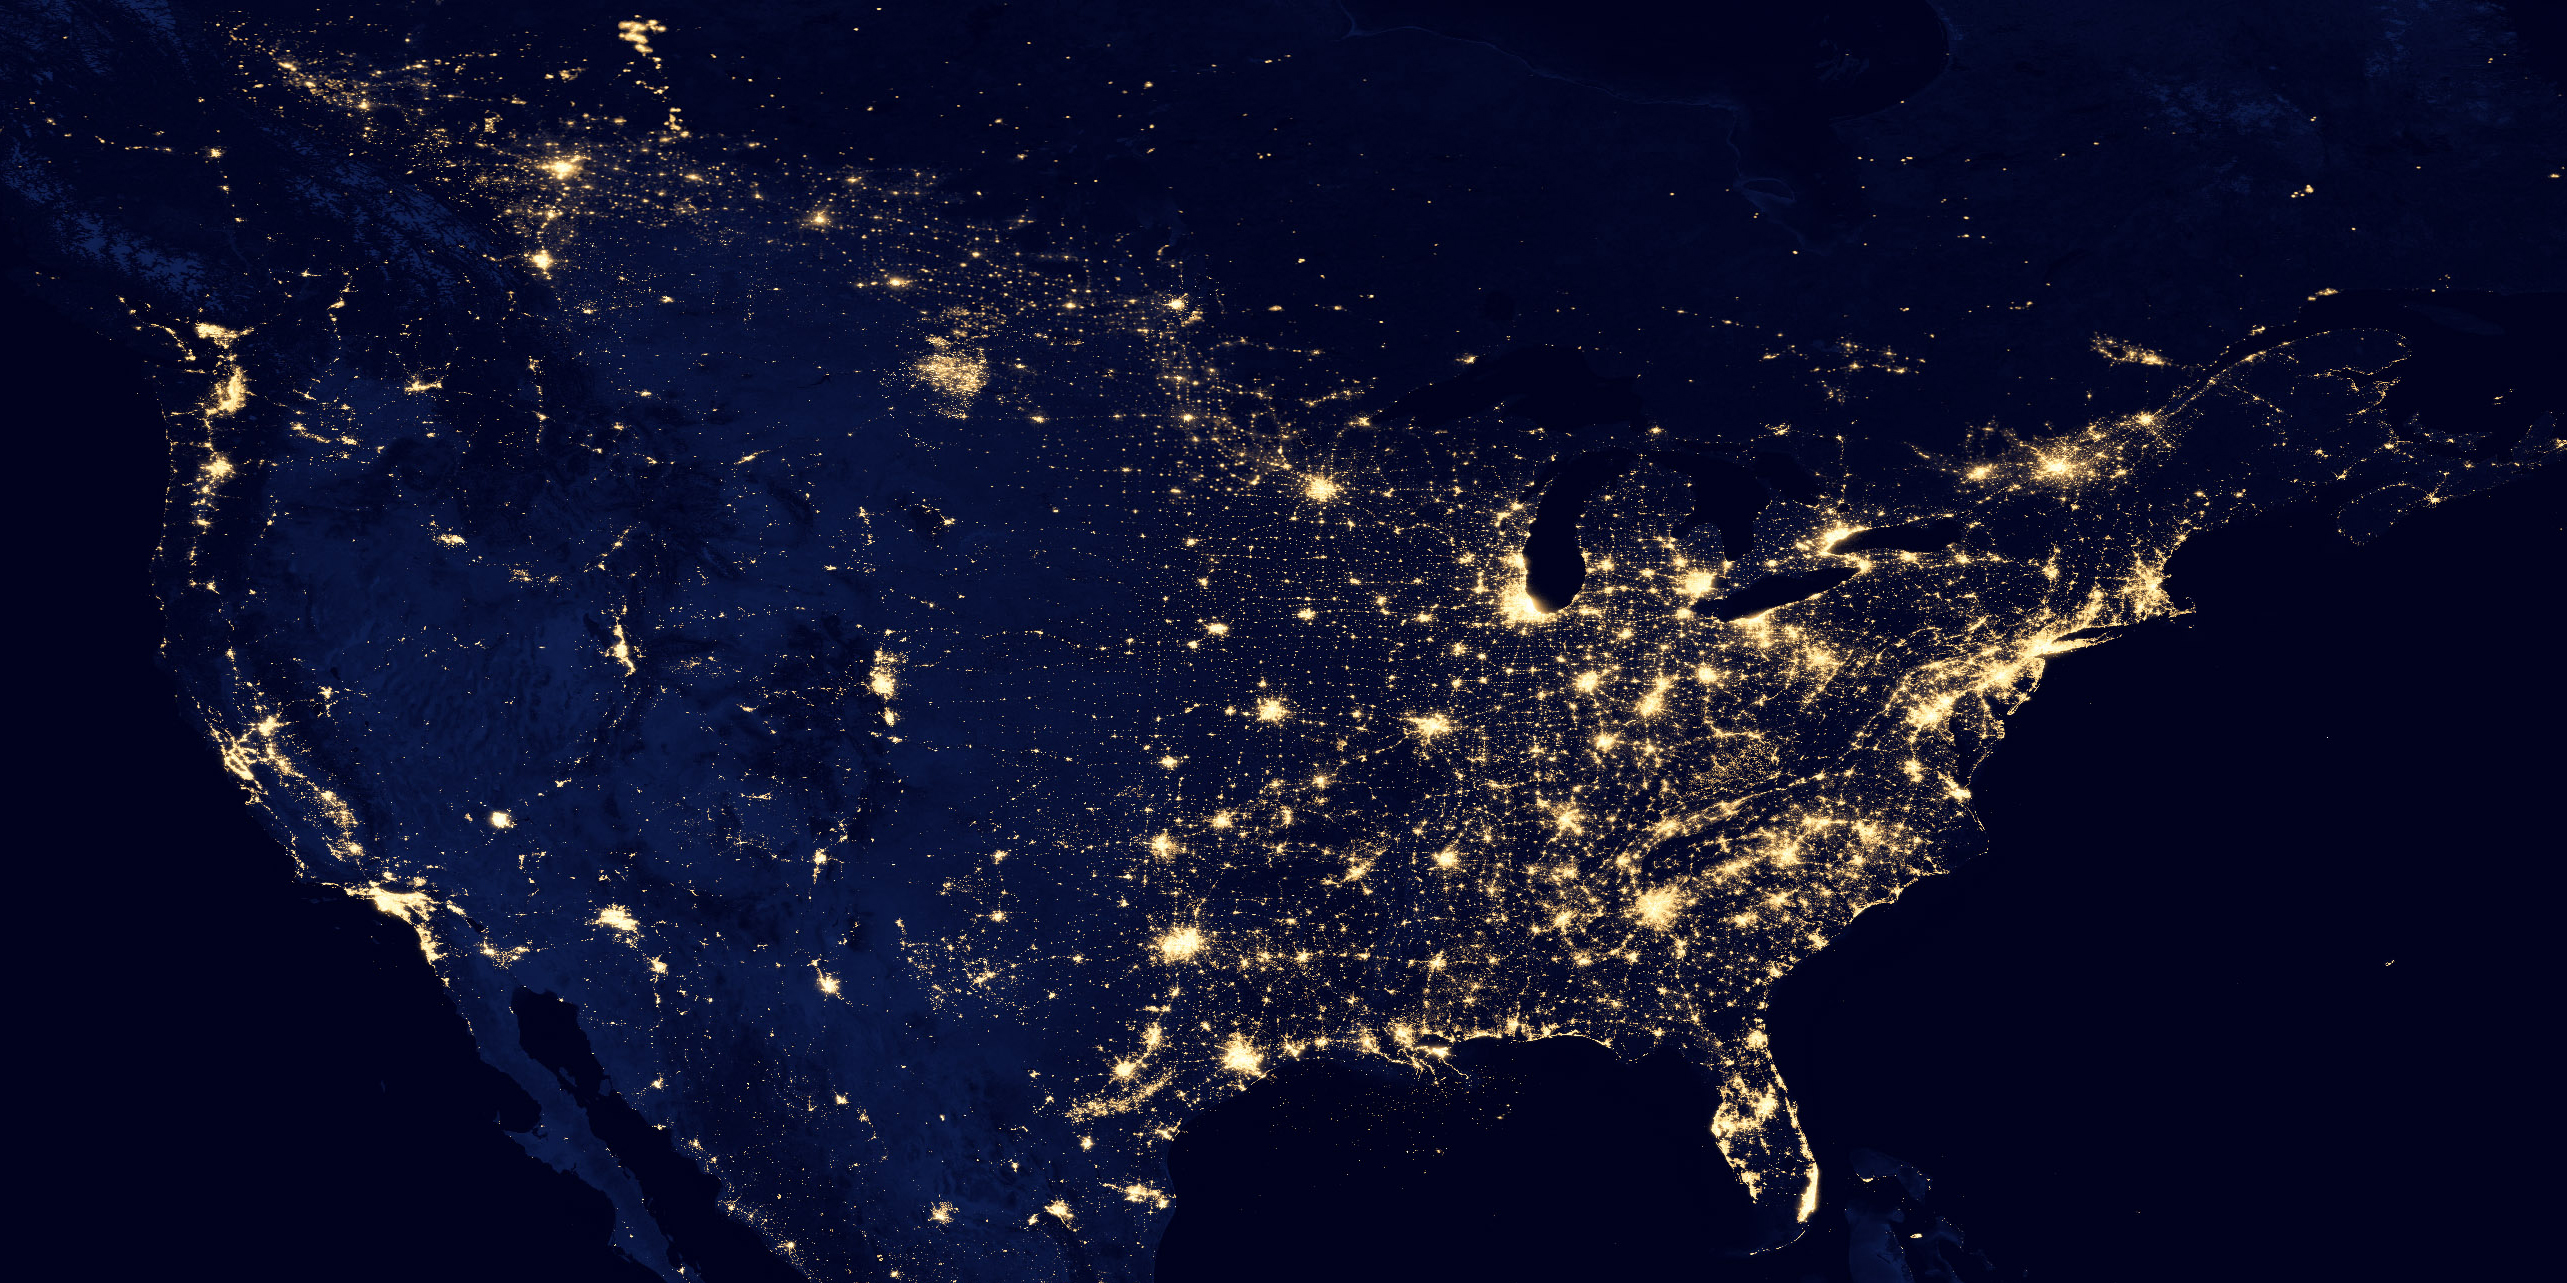
\includegraphics[width=8cm]{usa_by_night.jpg}\\
    \item{Densité en loi de puissance}
  \end{itemize}
\end{frame}

\begin{frame}
  \frametitle{Modèle de mobilité}
  \begin{itemize}
    \item{Nombre de joueurs}
    \item{Traversabilité des zones
      \\[1mm]\begin{center}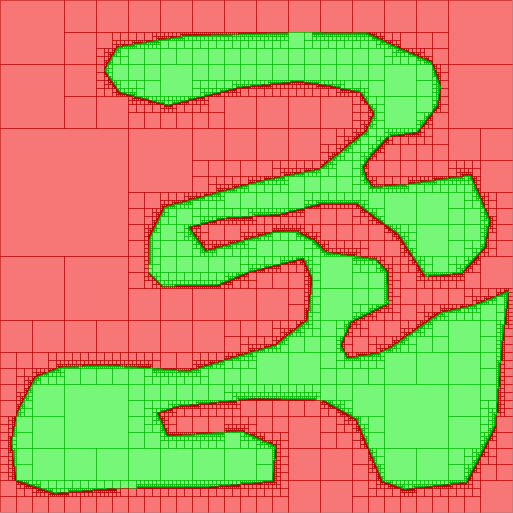
\includegraphics[width=6cm]{zones.png}\end{center}~
      \hspace{1cm}$\Rightarrow$ Nécessité de Pathfinding}
  \end{itemize}
\end{frame}

\begin{frame}
  \frametitle{Simulation}
  \begin{itemize}
    \item{4 types d'algorithmes}
    \begin{itemize}
      \item{Interest Management}
      \item{Replication Management}
      \item{Transfer Management}
      \item{Server Management\vspace{0.5cm}}
    \end{itemize}
    \item{Wrapper Simgrid\\[1mm]\hspace{1cm}$\Rightarrow$ Permet de passer plus facilement à un prototype}
  \end{itemize}
\end{frame}

\begin{frame}
  \frametitle{Tests}
  \begin{itemize}
    \item{Scénario 1\\[1mm]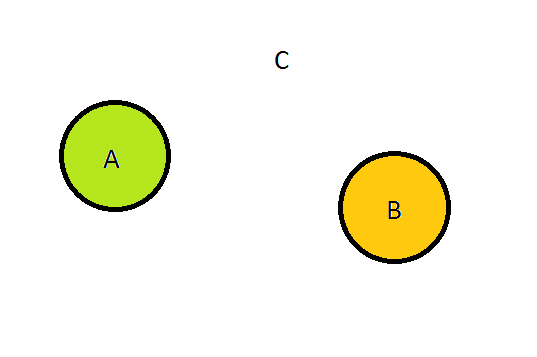
\includegraphics[width=5cm]{scenario_1.png}}
    \item{Scénario 2\\[1mm]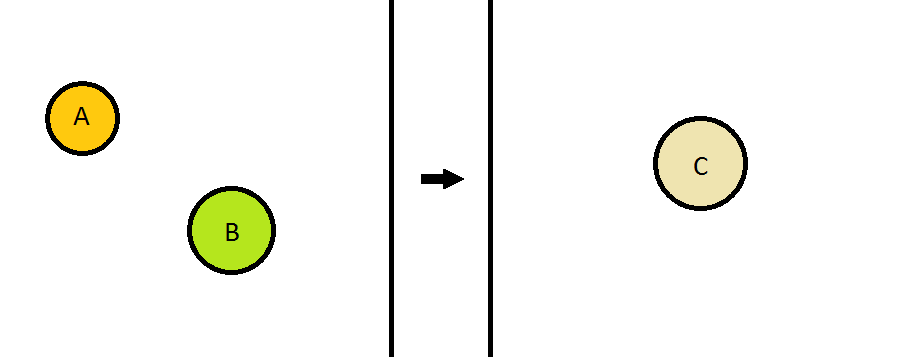
\includegraphics[width=6cm]{scenario_2.png}}
  \end{itemize}
\end{frame}

\begin{frame}
  \frametitle{Conclusion}
  \begin{itemize}
  \item{Outils pour la thèse}
    \begin{itemize}
      \item{Générateur de traces}
      \item{Simulateur suffisamment générique\vspace{0.8cm}}
    \end{itemize}
    \item{Travaux futurs}
    \begin{itemize}
      \item{Meilleur modèle de mobilité}
      \item{Architecture hybride}
    \end{itemize}
  \end{itemize}
\end{frame}

\setbeamertemplate{navigation symbols}{
}

\begin{frame}
  \frametitle{Support questions}
  \framesubtitle{Symétrie JPS}
  \centering
  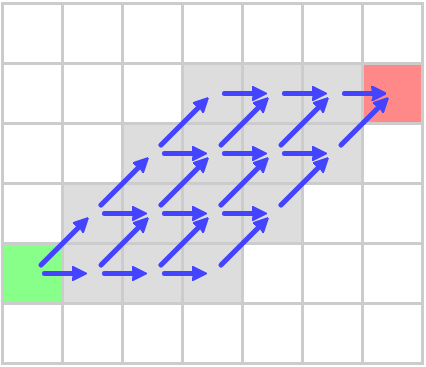
\includegraphics[width=7cm]{symetrie_JPS.png}
\end{frame}
\begin{frame}
  \frametitle{Support questions}
  \framesubtitle{Explication JPS}
  \centering
  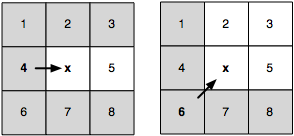
\includegraphics[width=7cm]{explo_jps.png}\\
  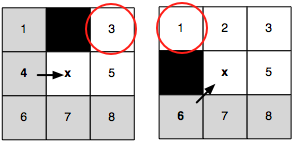
\includegraphics[width=7cm]{jmp_point_jps.png}
\end{frame}
\begin{frame}
  \frametitle{Support questions}
  \framesubtitle{Evolution nombre de joueurs}
  \centering
  \framebox{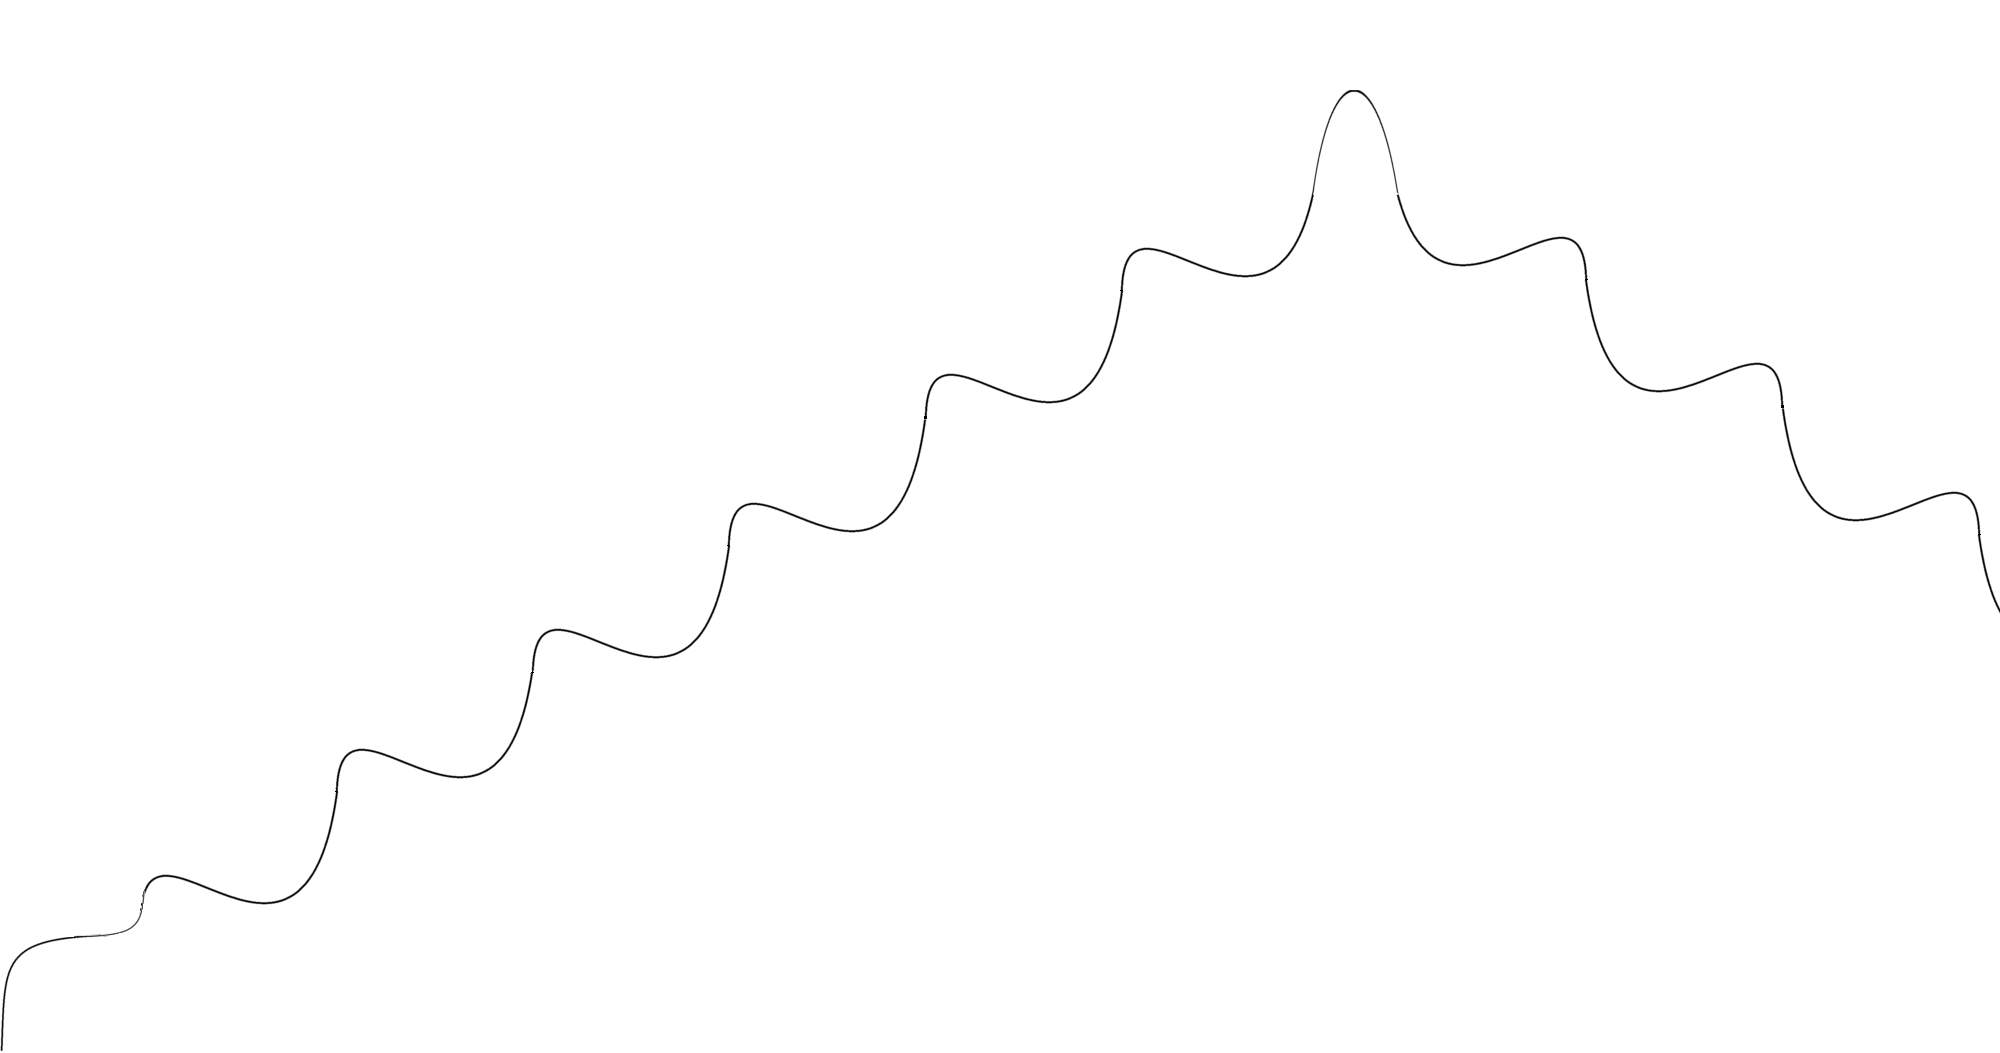
\includegraphics[width=7cm]{nbre_joueurs.png}}\\[1cm]
  \'Evolution du nombre de joueurs en fonction du temps
\end{frame}
\begin{frame}
  \frametitle{Support questions}
  \framesubtitle{Capture écran}
  \centering
  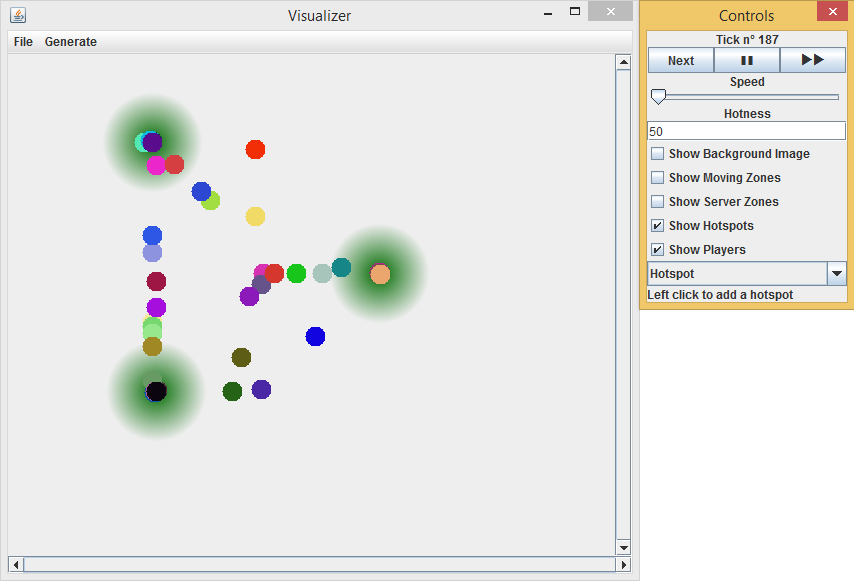
\includegraphics[width=9cm]{capture_ecran.png}
\end{frame}
\begin{frame}
  \frametitle{Support questions}
  \framesubtitle{Répartition autour d'un hotspot}
  \centering
  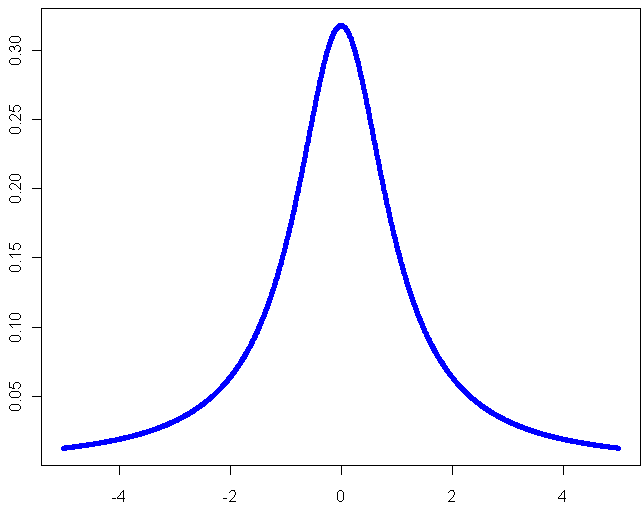
\includegraphics[width=7cm]{cauchy.png}\\
  Distribution de Cauchy
\end{frame}
\begin{frame}
  \frametitle{Support questions}
  \framesubtitle{Vols de Lévy}
  \centering
  \raisebox{-0.5\height}{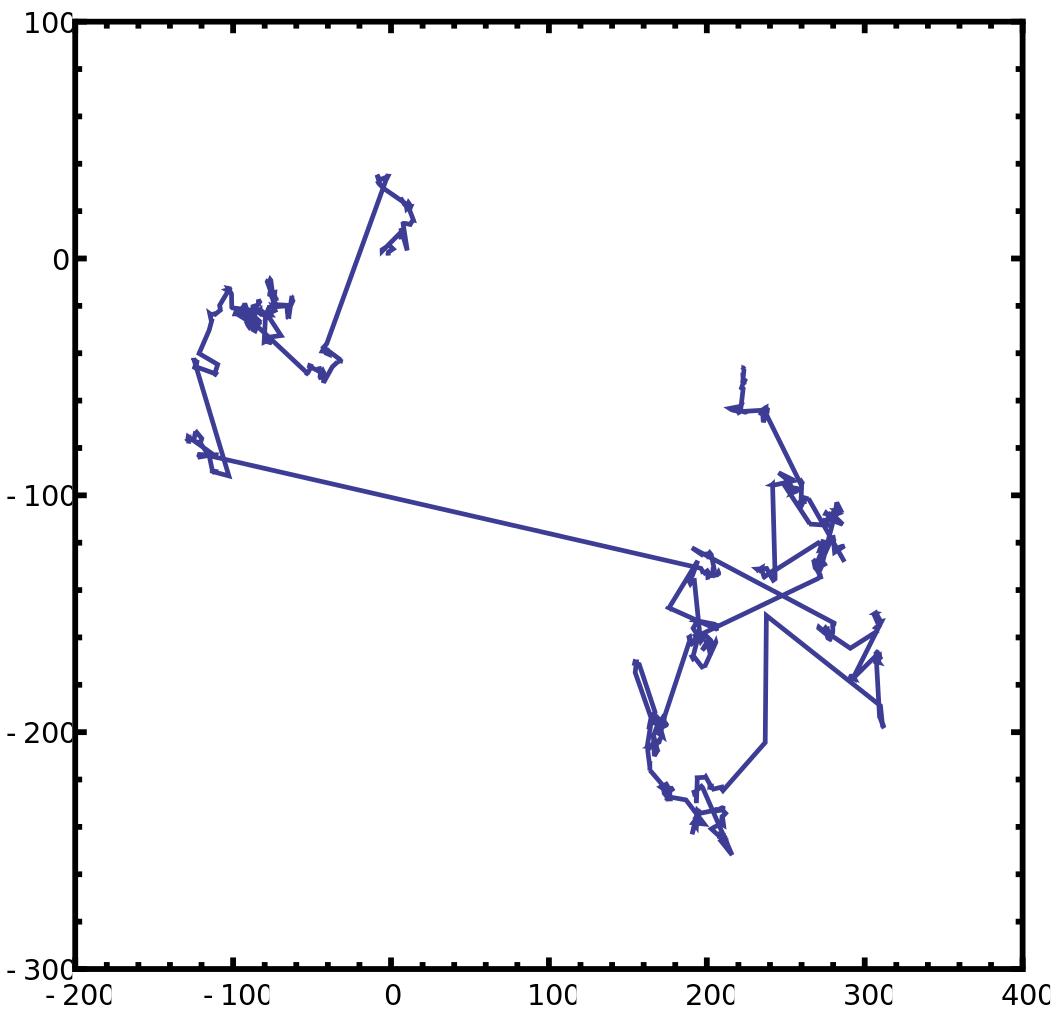
\includegraphics[width=4cm]{levy_1.png}}\hspace{1.2cm} Distribution de Cauchy\\
  \raisebox{-0.5\height}{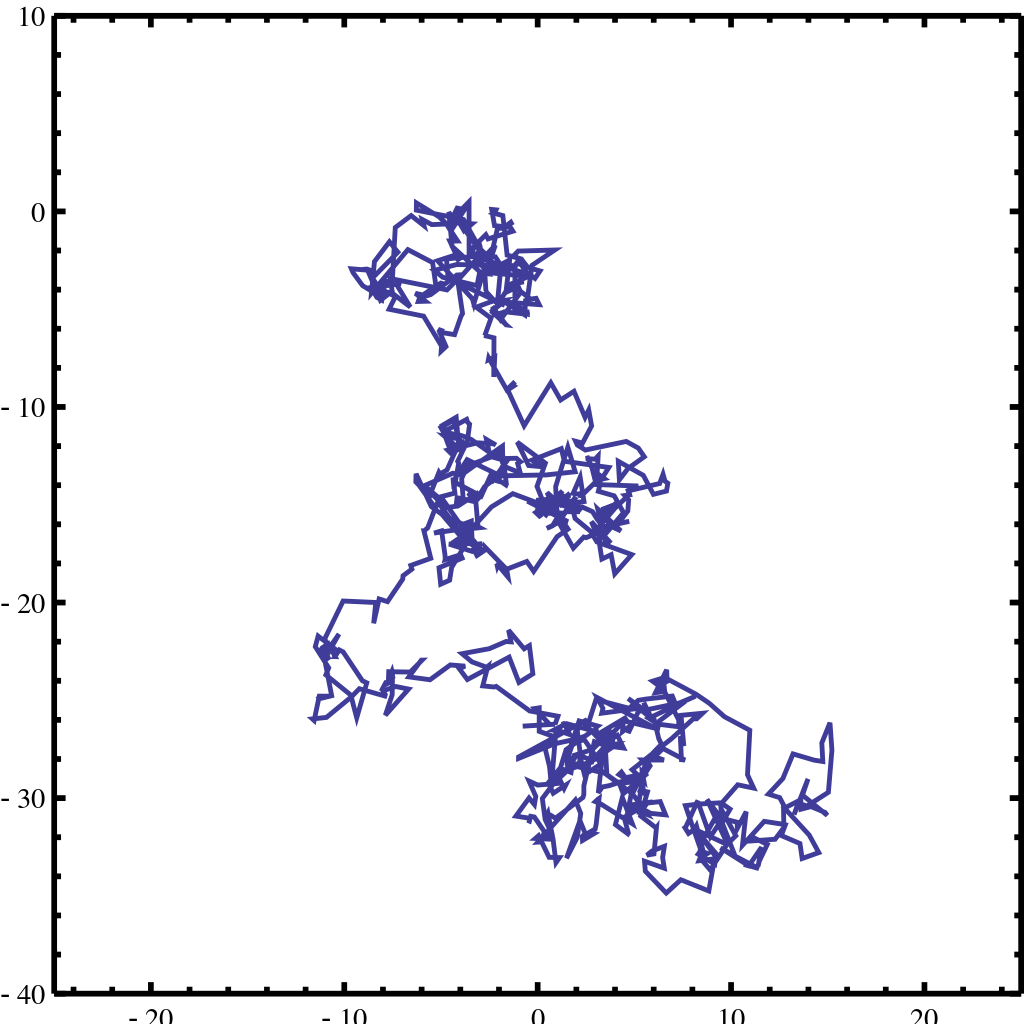
\includegraphics[width=4cm]{levy_2.png}}\hspace{1cm} Distribution normale
\end{frame}

\end{document}

